\emph{How do (management) scholars evaluate a standard natural experiment research
design?} According to Dunning (\cite*[][page 27]{dunning2012}), the validity of
a natural experiment should be assessed against three criteria (see Figure
\ref{fig:validity_framework}).  First, scholars should prove the random
nature of the treatment or, at least, defend the plausibility of as-if random.
In the \emph{randomized standard natural experiment}, it is
important that the assignment process is truly random. Although this may seem
obvious, this condition is sometimes violated, even in the context of lotteries
\parencite[e.g.,][]{Starr1997}. In the case of \emph{as-if randomization}, it
is vital the assignment process is: i) independent of
factors that are related to the outcome, and ii) not affected by unit's
self-selection into treatment or control conditions. As Dunning points out, the
researcher has to make a compelling case for this assertion (or refrain from
claiming he/she conducts a natural experiment). In-depth knowledge of the context (e.g.,
industry regulatory frameworks), qualitative evidence about the naturally
occurring event (e.g., a new law), and quantitative evidence at the event- and
unit-level are essential ingredients to defend the plausibility of
as-if random assignment, and, ultimately, to sustain the natural experiment.

Second, the naturally occurring event should reveal the wider
\emph{``theoretical, substantive, and/or policy issues''} \parencite[][page
29]{Dunning2012} that motivate the study. For example, the sudden, premature
death of a star scientist \parencite[][]{Azoulay2010} create the premises for a
natural experiment that quantifies the spill-over effect of collaborating with
academics who are prominent in their fields of research.

Finally, the statistical model should fit with the characteristics of the
naturally occurring event. In the case of a randomized standard natural
experiment, simplicity and transparency should take precedence in the data
analysis stage. Particularly, Neyman's potential outcomes framework
\parencite[][]{Splawa1990}, namely, a treated Vs. control mean comparison test,
should be used \emph{prima facie}. At the same time, some statistical
adjustments may be required even in presence of a random (or as-if random)
treatment. For example, the Stable-Unit-Treatment-Value-Assumption (SUTVA) may
be violated insofar as the treatment status of a unit $i$ interferes with the
potential outcome of unit j. Such a concern is central in the Belloc and
colleagues's \parencite*[][]{Belloc2016} study about the impact of earthquakes
on institutional change at the city-level in the Middle-Ages northern and
central Italy. Both the distribution and timing of earthquakes are random.
However, the probability a control city will move from autocratic regimes to
self-government is also a function of the information key actors are exposed to,
such as the transition choices treated neighboring cities make. In this case,
scholars may want to adopt some statistical adjustments to model the correlation
of residuals induced by the geographical proximity of any pair of units.

\begin{figure}
    \large
    \sffamily
    \begin{small}
        \label{fig:validity_framework}
        \begin{center}
            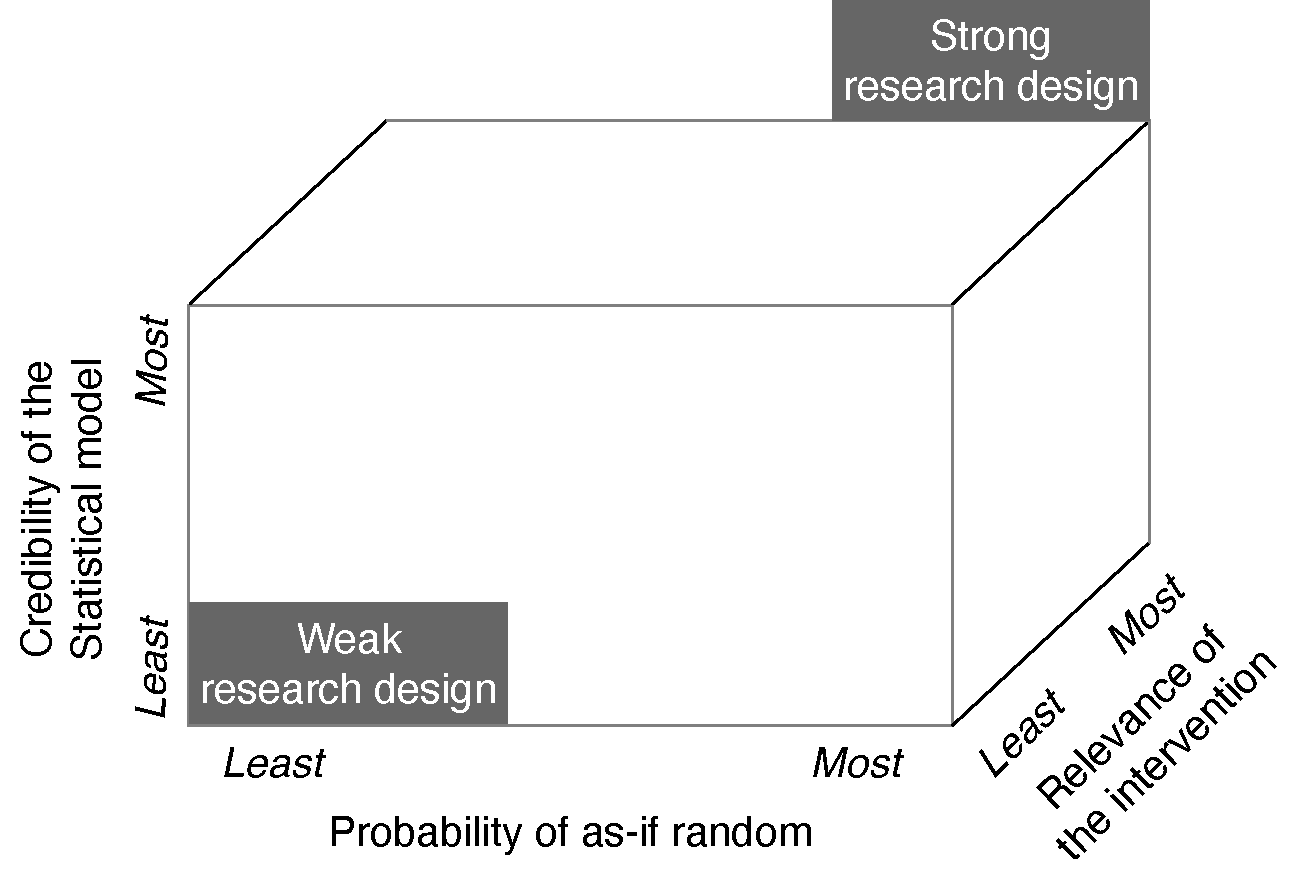
\includegraphics[width=0.80\textwidth]{exhibits/validity_framework.pdf}
        \end{center}
    \end{small}
    \caption{Visual representation of Dunning's validity framework \parencite[][page]{dunning2012}}.
\end{figure}
